\documentclass{article}
\usepackage{graphicx} % Required for inserting images
\usepackage{hyperref}
\usepackage{longtable}

\title{How to Arduino}
\author{Olaf Hafsmo}
\date{June 2023}

\begin{document}

\maketitle
\newpage
\section*{Formål}
Hovedformålet til denne laben er å innføre gode rutiner ved arbeid på mikrokontrollere.  Videre skal studentene få en innføring i gode praksiser ved prototypearbeid, med hovedfokus på sikkerhet, nøyaktighet og repeterbarhet.

\section*{Forkunnskaper}
Frem til nå skal dere ha hatt grunnleggende kretsteori, samt være kjent med Arduino IDE og grunnleggende programmering. Dette heftet etterstreber å inneha all kunnskap, samt kilder til ekstern litteratur. Ekstern litteratur skal altså ikke være nødvendig for å fullføre laben, men det anbefales å benytte dersom behov.

\section*{Bakenforliggende teori}

\subsection*{Kretsskjema}
Alt godt ingeniørarbeid starter med en tegning, en god tegning starter med gode standarder. NEK 144:2017 er tilgjengelig for studenter på NTNU ved \href{https://handle.standard.no/no/Nettbutikk/produktkatalogen/Produktpresentasjon/?ProductID=923060}{standard.no} og inneholder de fleste symboler man trenger. Dersom du mangler et symbol er NEK 144:2017 hentet fra IEC 60617 DB som er mer utfyllende.
\\
Det anbefales sterkt å tegne kretsskjema på rutenett eller annet koordinatsystem.
\\
\\
Generelle regler for å imøtekomme NEK 400:2017
\begin{itemize}
    \item Alle ledninger er horisontale eller vertikale, med unntak av retningsindikerte forbindelser, men det er teknisk sett et symbol.
    \item Alle "svinger" er skarpe 90 grader.
    \item Alle termineringspunkter merkes med helfarget punkt.
    \item Alle symboler skal ha unike navn, en vanlig praksis er <xx00> hvorav <xx> er bokstavkode og <00> er løpenummer.
    \item Alle symboler er hentet fra IEC 60617 eller sammensatte ut fra normen, dersom det ikke lar seg gjøre skal det være tydelig forklart hva symbolets funksjon er.
    \item Alt utstyr som er montert i samme kapsling skal omsluttes med stiplet kant, som skal ha et unikt navn merket i øvre venstre hjørne av det stiplede feltet.
\end{itemize}

\subsubsection*{Vanlige symboler}
\begin{center}
    \begin{longtable}{c}
    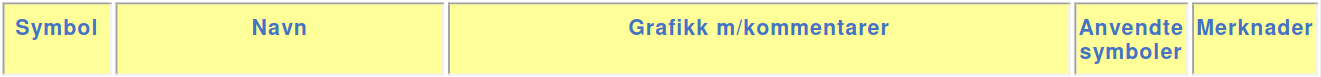
\includegraphics[width=0.9\textwidth]{bilder/header.png}\\
    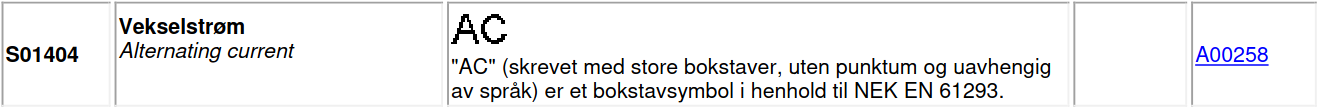
\includegraphics[width=0.9\textwidth]{bilder/s01404.png}\\
    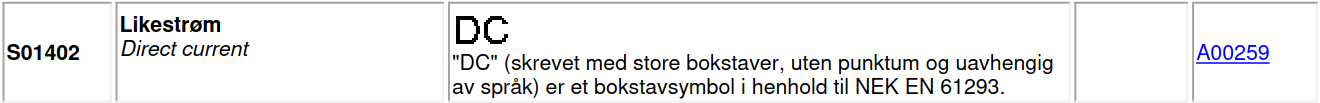
\includegraphics[width=0.9\textwidth]{bilder/s01402.png}\\
    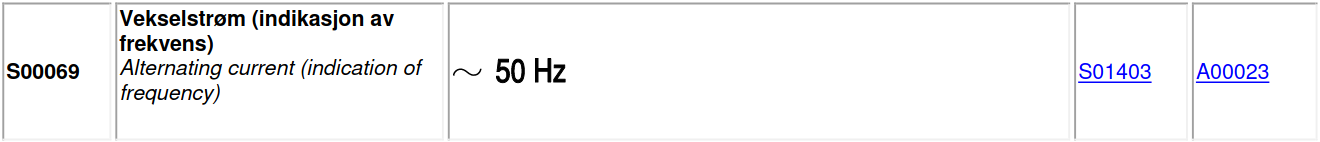
\includegraphics[width=0.9\textwidth]{bilder/s00069.png}\\
    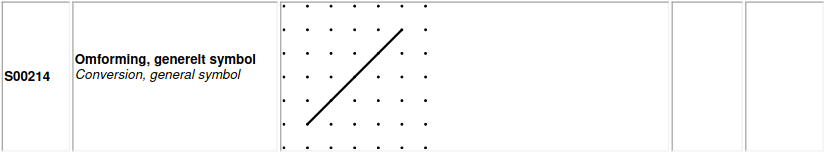
\includegraphics[width=0.9\textwidth]{bilder/s00214.png}\\
    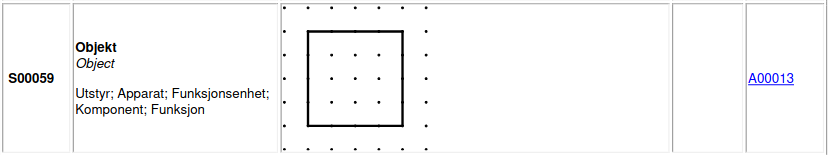
\includegraphics[width=0.9\textwidth]{bilder/s00059.png}\\
    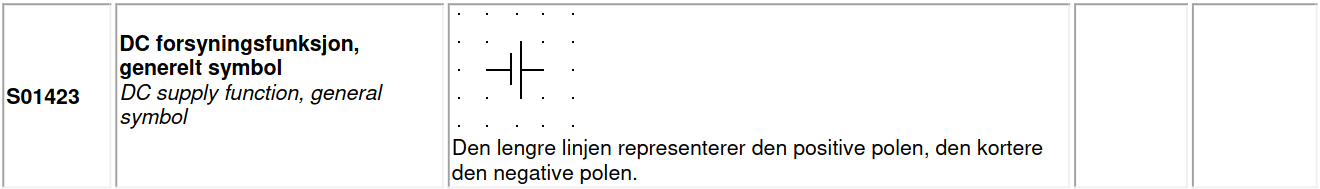
\includegraphics[width=0.9\textwidth]{bilder/s01423.png}\\
    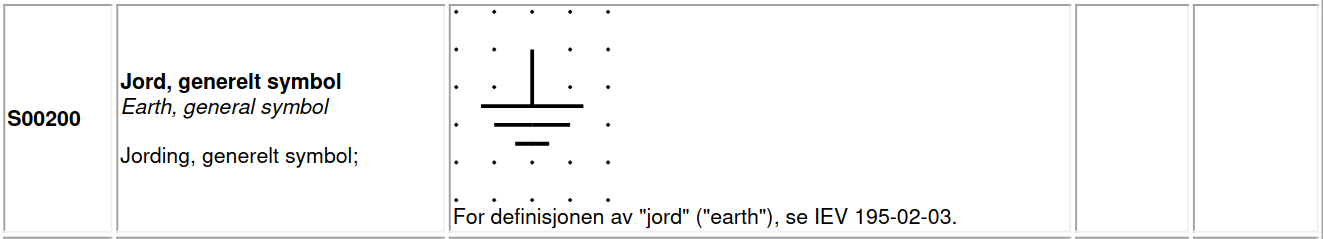
\includegraphics[width=0.9\textwidth]{bilder/s00200.png}\\
    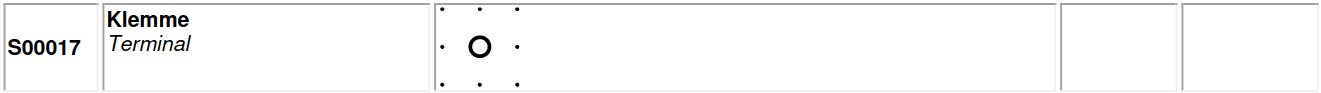
\includegraphics[width=0.9\textwidth]{bilder/s00017.png}\\
    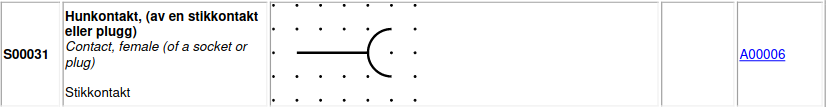
\includegraphics[width=0.9\textwidth]{bilder/s00031.png}\\
    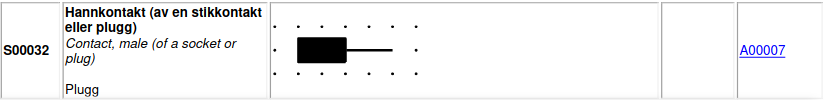
\includegraphics[width=0.9\textwidth]{bilder/s00032.png}\\
    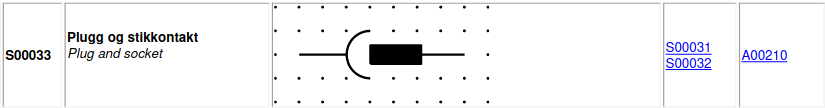
\includegraphics[width=0.9\textwidth]{bilder/s00033.png}\\
    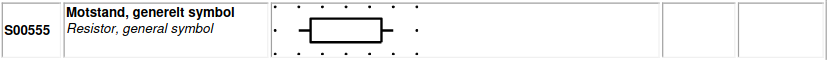
\includegraphics[width=0.9\textwidth]{bilder/s00555.png}\\
    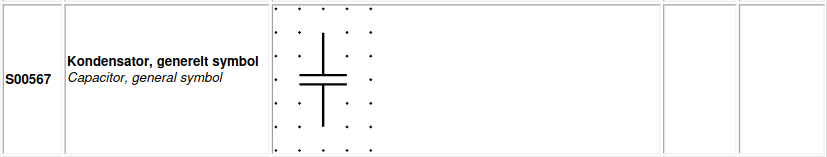
\includegraphics[width=0.9\textwidth]{bilder/s00567.png}\\
    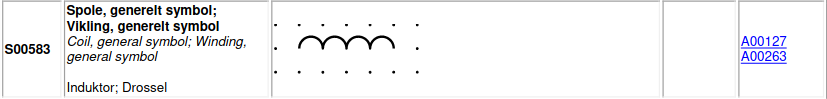
\includegraphics[width=0.9\textwidth]{bilder/s00583.png}\\
    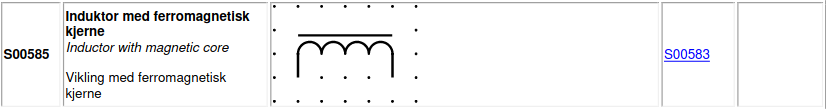
\includegraphics[width=0.9\textwidth]{bilder/s00585.png}\\
    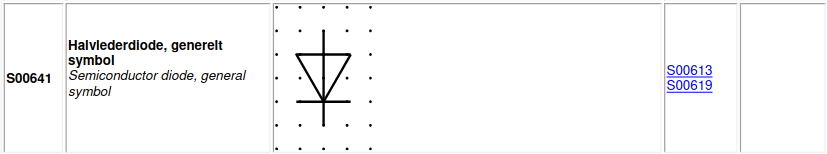
\includegraphics[width=0.9\textwidth]{bilder/s00641.png}\\
    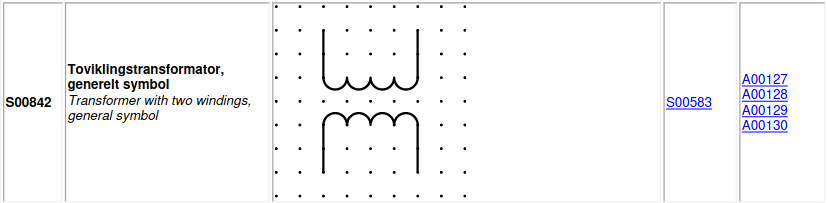
\includegraphics[width=0.9\textwidth]{bilder/s00842.png}\\
    \end{longtable}
\end{center}
\subsubsection*{Vanlige tilleggssymboler}
\begin{center}
    \begin{longtable}{c}
        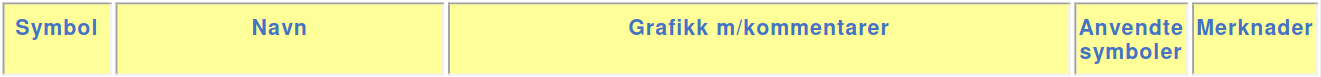
\includegraphics[width=0.9\textwidth]{bilder/header.png}\\
        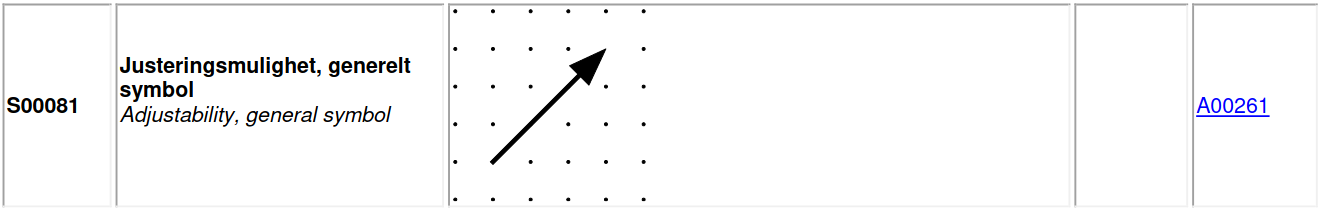
\includegraphics[width=0.9\textwidth]{bilder/s00081.png}\\
        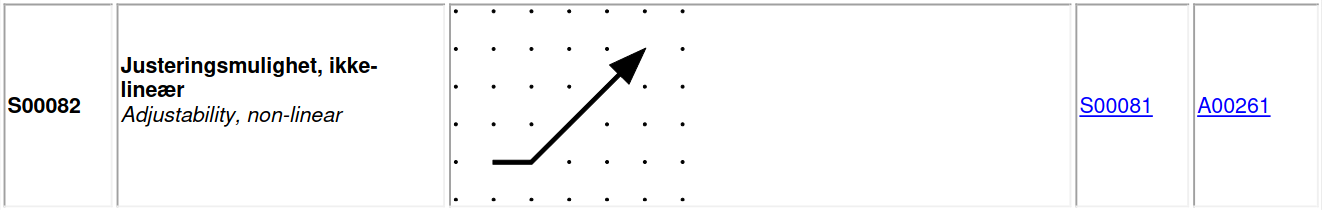
\includegraphics[width=0.9\textwidth]{bilder/s00082.png}\\
        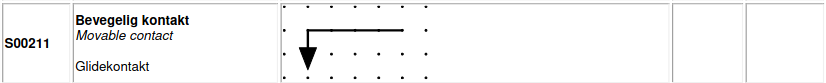
\includegraphics[width=0.9\textwidth]{bilder/s00211.png}\\
        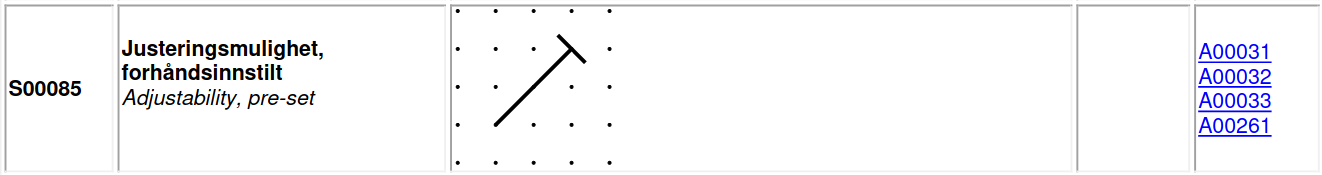
\includegraphics[width=0.9\textwidth]{bilder/s00085.png}\\
        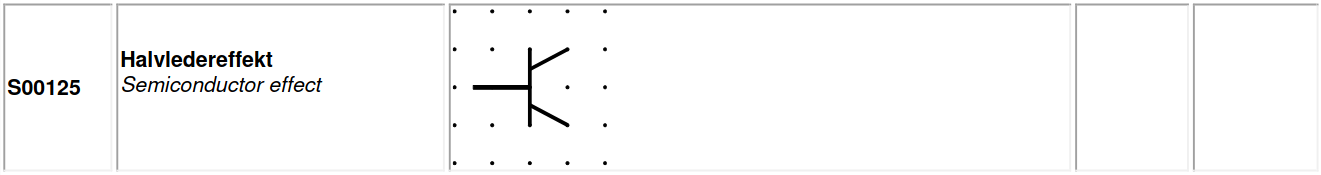
\includegraphics[width=0.9\textwidth]{bilder/s00125.png}\\
        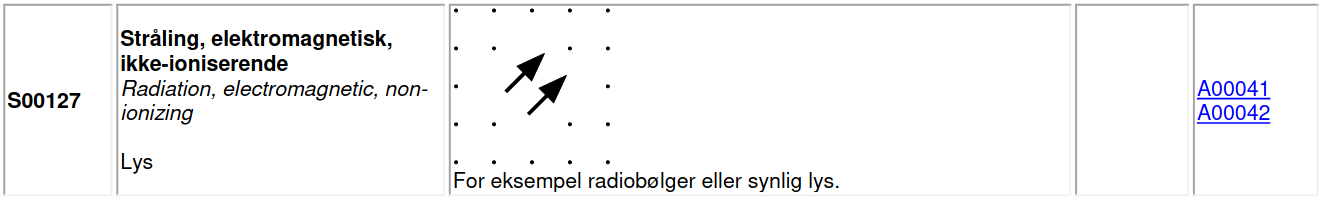
\includegraphics[width=0.9\textwidth]{bilder/s00127.png}\\
        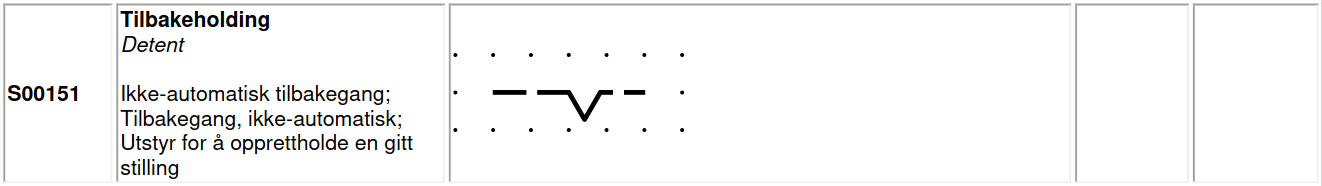
\includegraphics[width=0.9\textwidth]{bilder/s00151.png}\\
        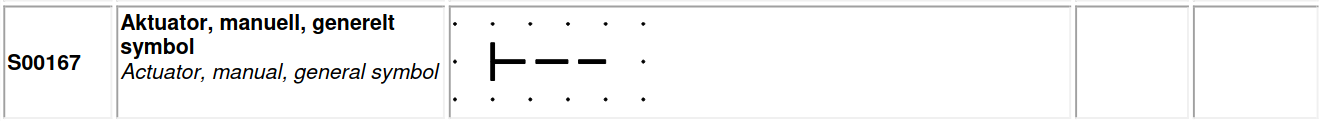
\includegraphics[width=0.9\textwidth]{bilder/s00167.png}\\
        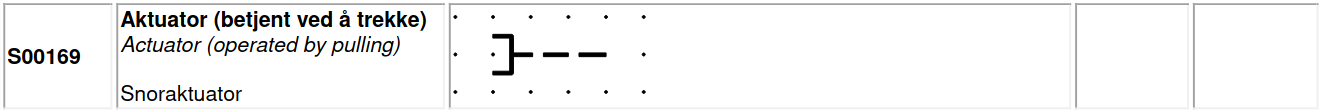
\includegraphics[width=0.9\textwidth]{bilder/s00169.png}\\
        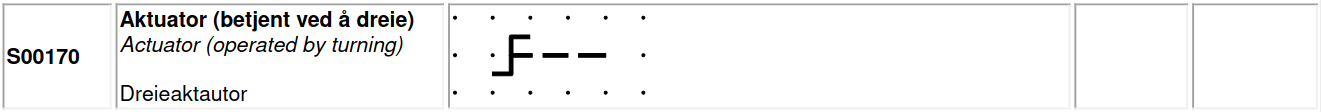
\includegraphics[width=0.9\textwidth]{bilder/s00170.png}\\
        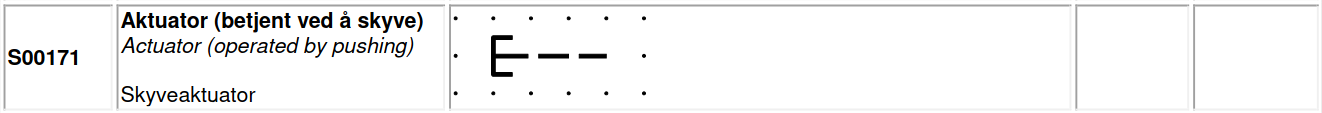
\includegraphics[width=0.9\textwidth]{bilder/s00171.png}\\
        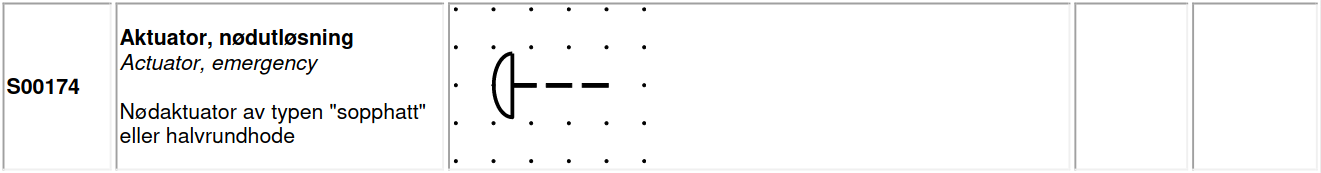
\includegraphics[width=0.9\textwidth]{bilder/s00174.png}\\
        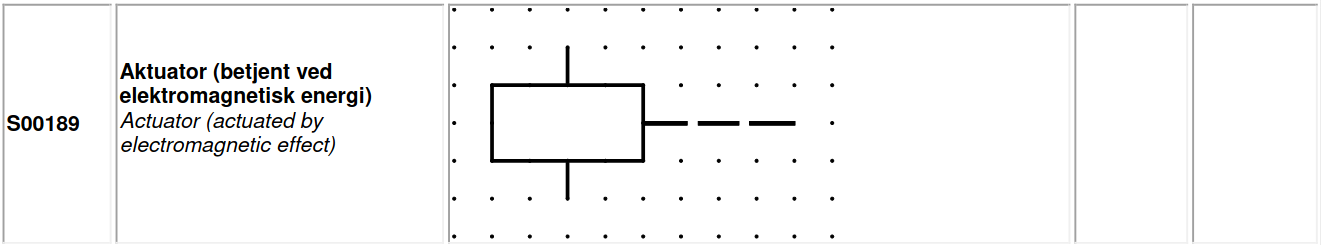
\includegraphics[width=0.9\textwidth]{bilder/s00189.png}\\
        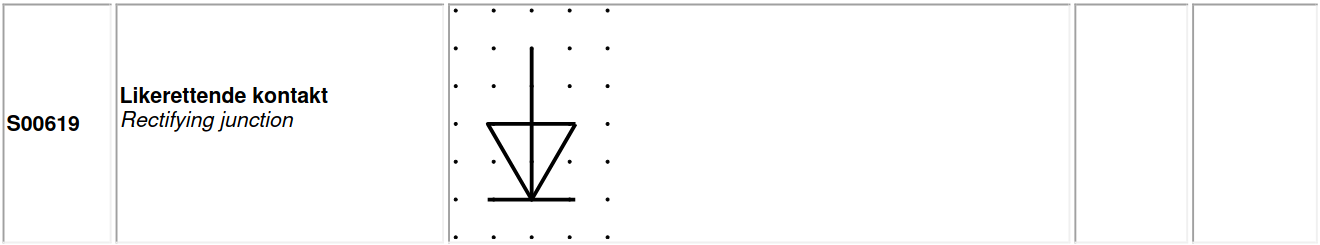
\includegraphics[width=0.9\textwidth]{bilder/s00619.png}\\
        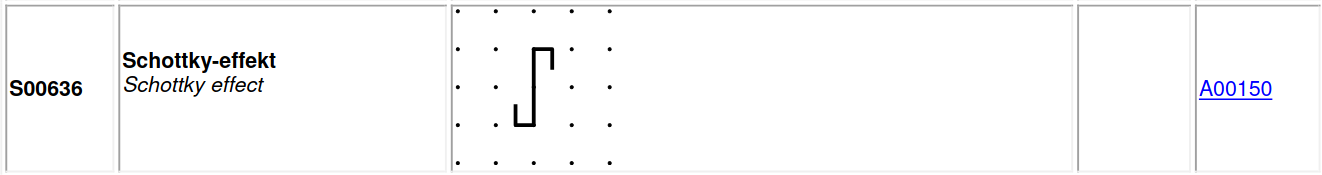
\includegraphics[width=0.9\textwidth]{bilder/s00636.png}\\
        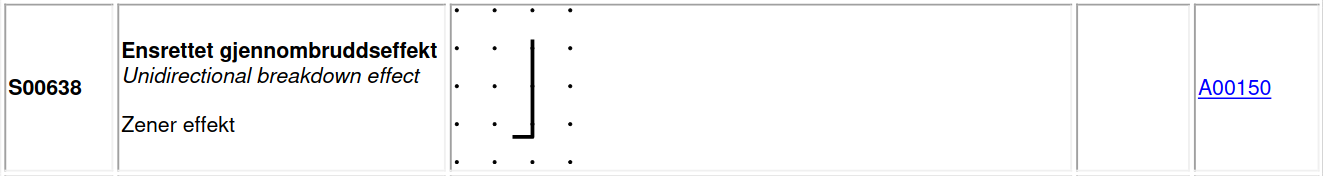
\includegraphics[width=0.9\textwidth]{bilder/s00638.png}\\
        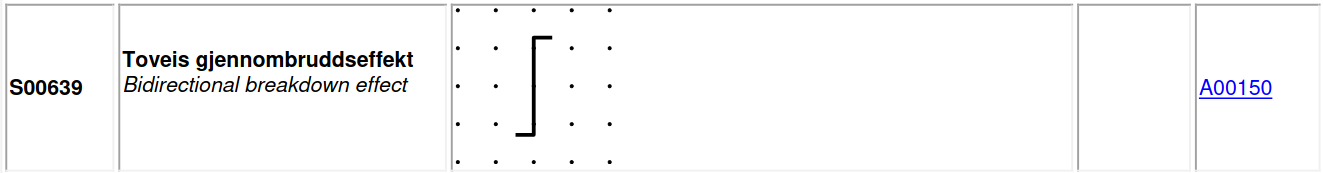
\includegraphics[width=0.9\textwidth]{bilder/s00639.png}\\
        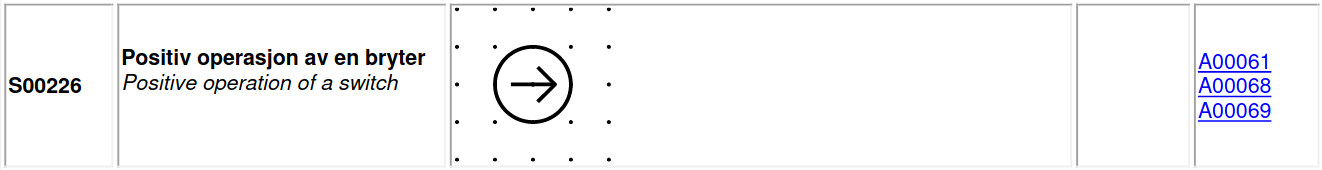
\includegraphics[width=0.9\textwidth]{bilder/s00226.png}\\
        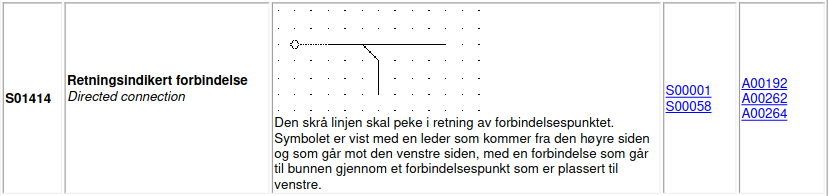
\includegraphics[width=0.9\textwidth]{bilder/s01414.png}\\
       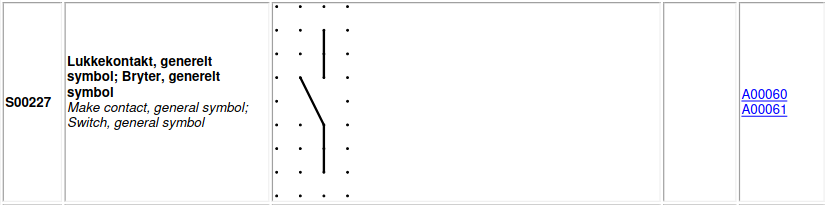
\includegraphics[width=0.9\textwidth]{bilder/s00227.png}\\
        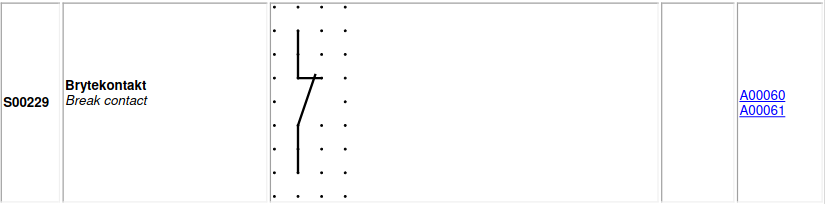
\includegraphics[width=0.9\textwidth]{bilder/s00229.png}\\
        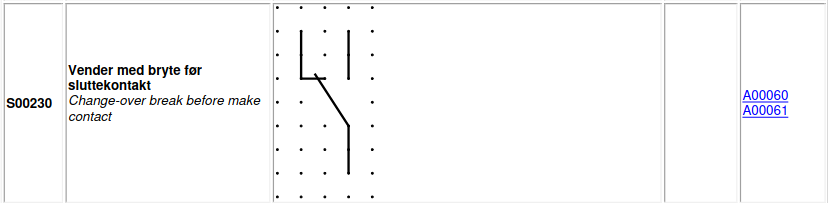
\includegraphics[width=0.9\textwidth]{bilder/s00230.png}\\
        
    \end{longtable}
\end{center}
\subsubsection*{Hvordan sette sammen symboler}
Det er et par måter man kan sette sammen symboler etter NEK400:2017. Vi skal se på de to vanligste måtene. Det er viktig fra normens side at symbolikken enklegjør det fysiske domenet; herunder koblingsveier og betjeningsmåte. Videre skal det elektrotekniske komme frem; herunder signalkondisjonering og sensorer.

Ofte vil man se sammensatte symboler, der man benytter et grunnsymbol som beskriver hovedfunksjonen, og deretter legger på tilleggssymboler for å gi mer info om bruksbetingelser. Dette er vanligst i det fysiske domenet. Se eksempel hentet fra NEK144:2017.\\
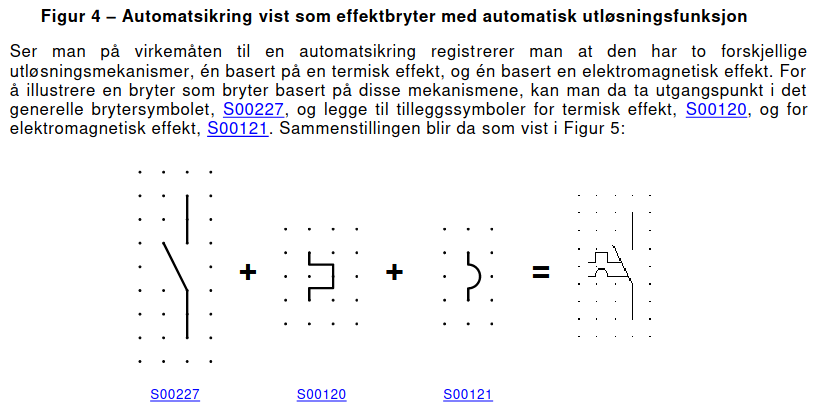
\includegraphics[width=0.9\textwidth]{bilder/eksempel 1 symbolsammensetning.png}\\

En annen vanlig praksis er at man tegner en boks rundt tilleggssymbolene og på dette viset beskriver funksjonalitet. Dette er vanligst i det elektrotekniske domenet. Se eksempel hentet fra NEK144:2017.\\
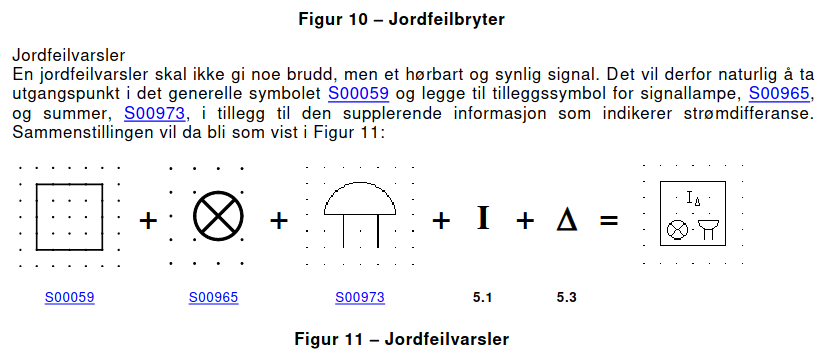
\includegraphics[width=0.9\textwidth]{bilder/eksempel 2 symbolsammensetning.png}\\

\subsection*{kabelberegninger}

Som utgangspunkt antar vi PVC isolert flerledet kobberkabel, forlagt i luft ved 30$^\circ$C, og maksimalt strømtrekk 16A. 
\\
\\
$I=A\cdot S^m - B\cdot S^n$\\
Hvorav\\
I=maksimalt strømtrekk kabel\\
A=16.8\\
S=tverrsnitt [$mm^2$]\\
m=0.627\\
B=0\\
n=0


Videre må man ta hensyn til omgivelsestemperatur og nærføring. Dette gjøres ved å gange inn koeffisienter hentet fra underlagte tabeller.
\\
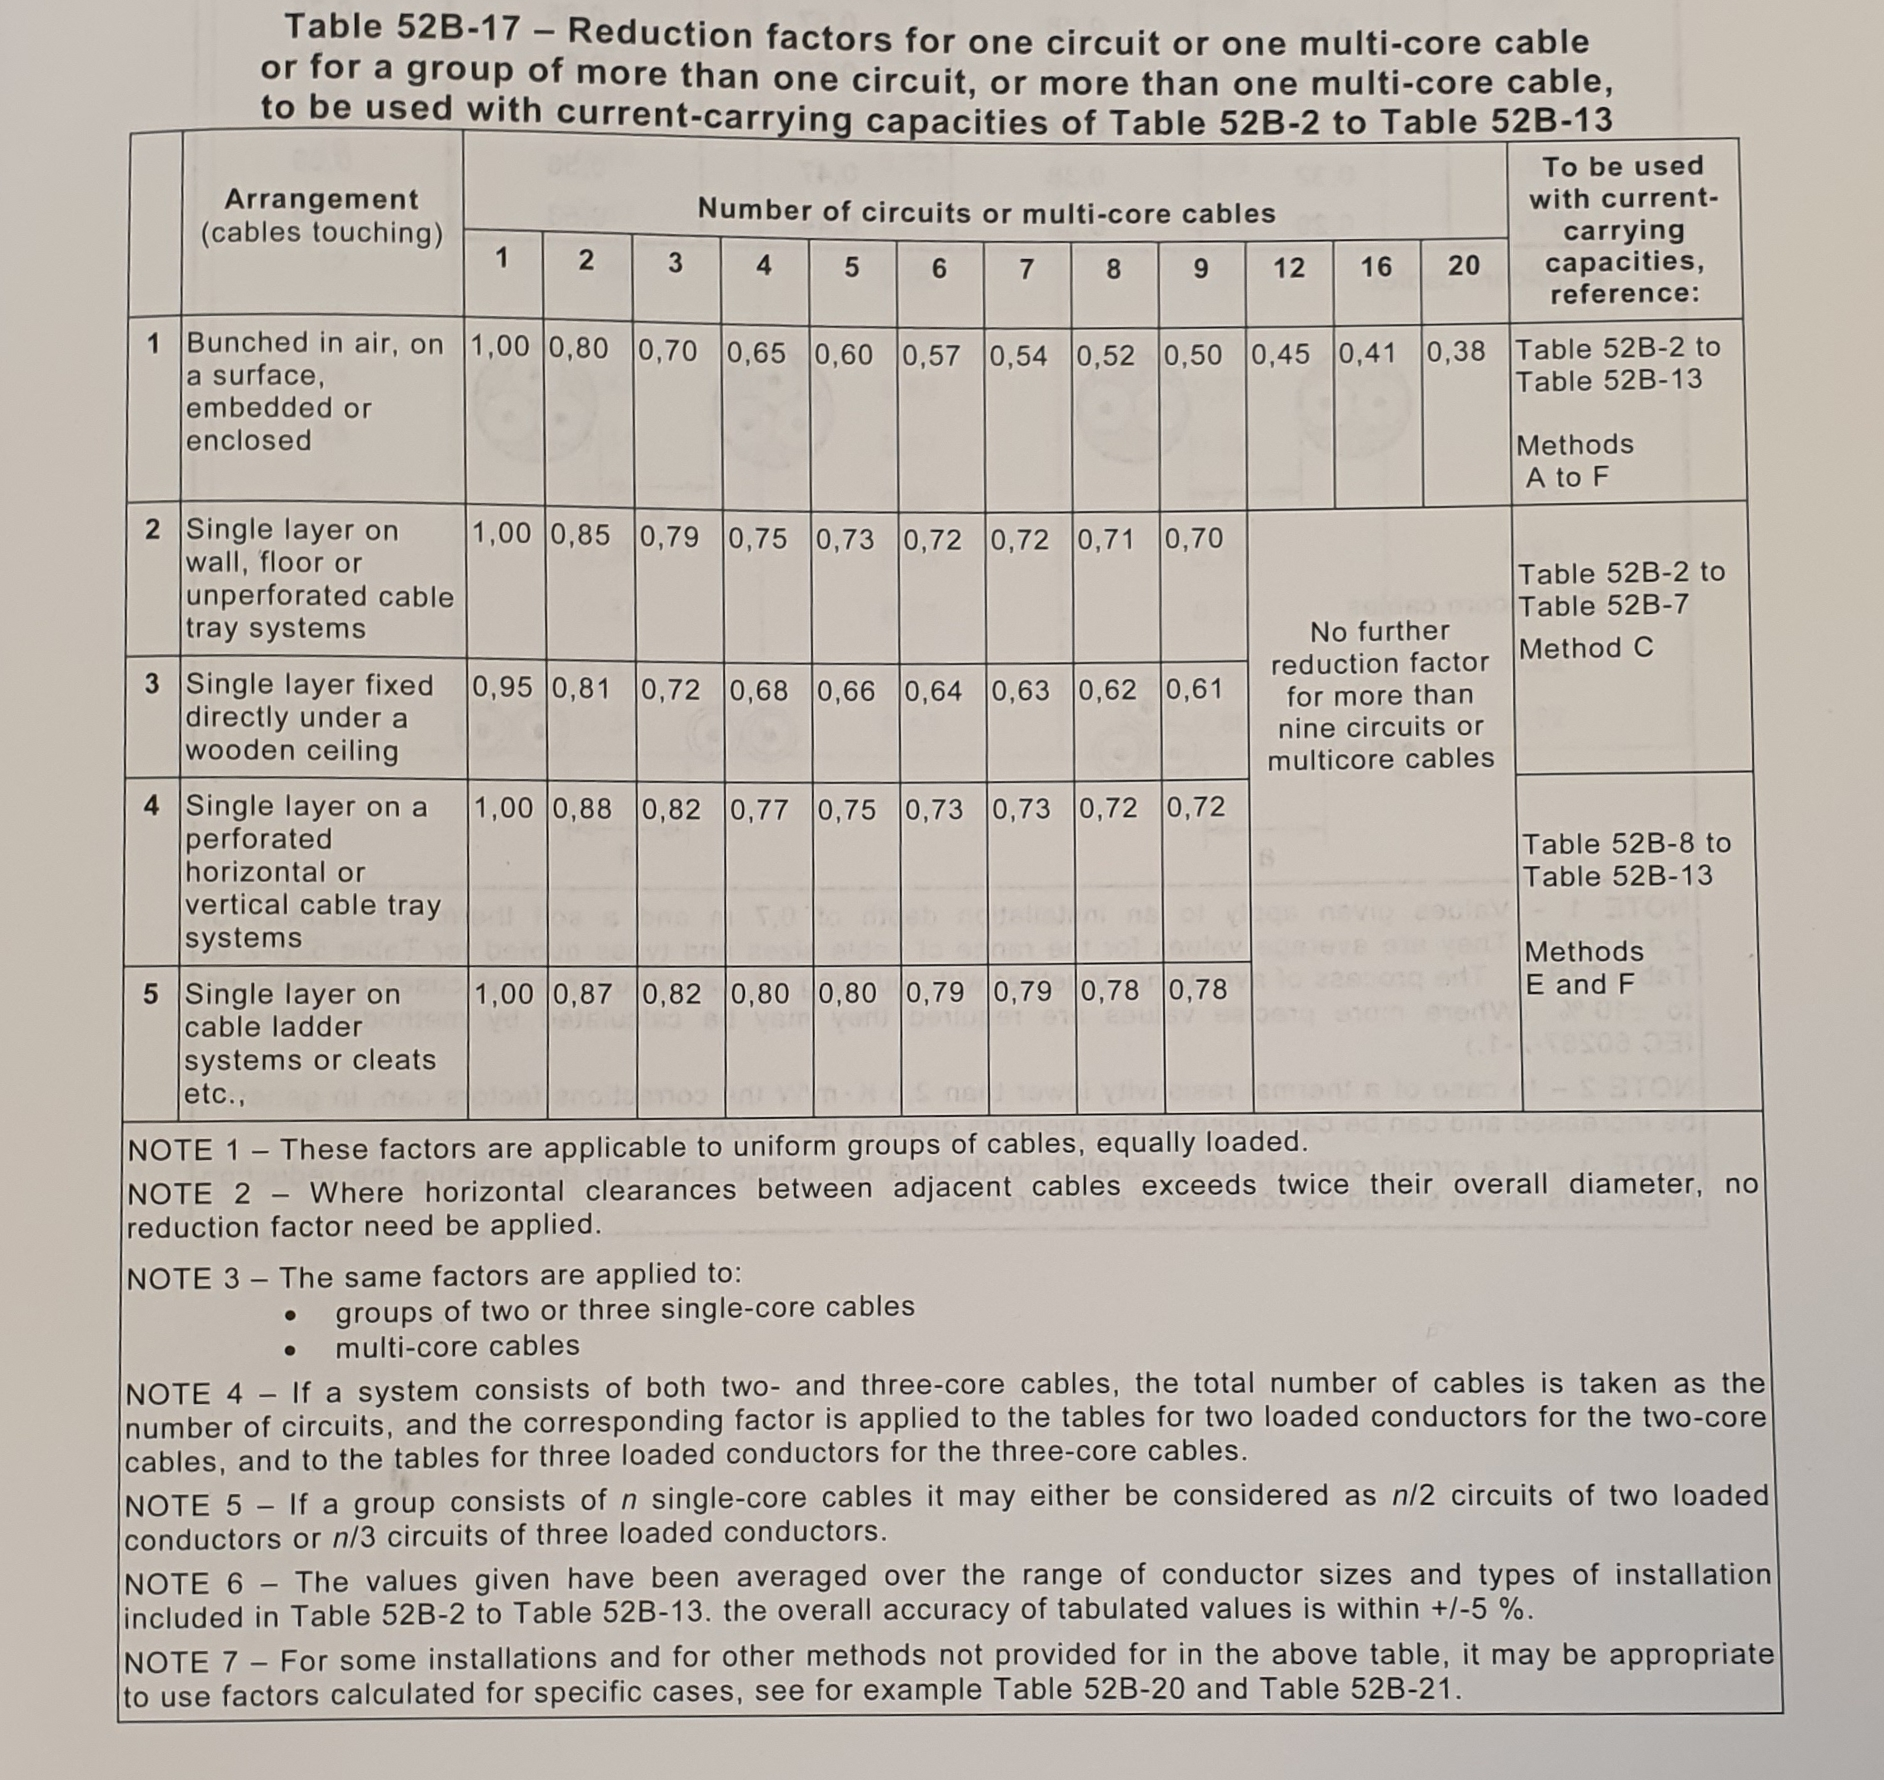
\includegraphics[width=0.9\textwidth]{bilder/close.jpg}\\
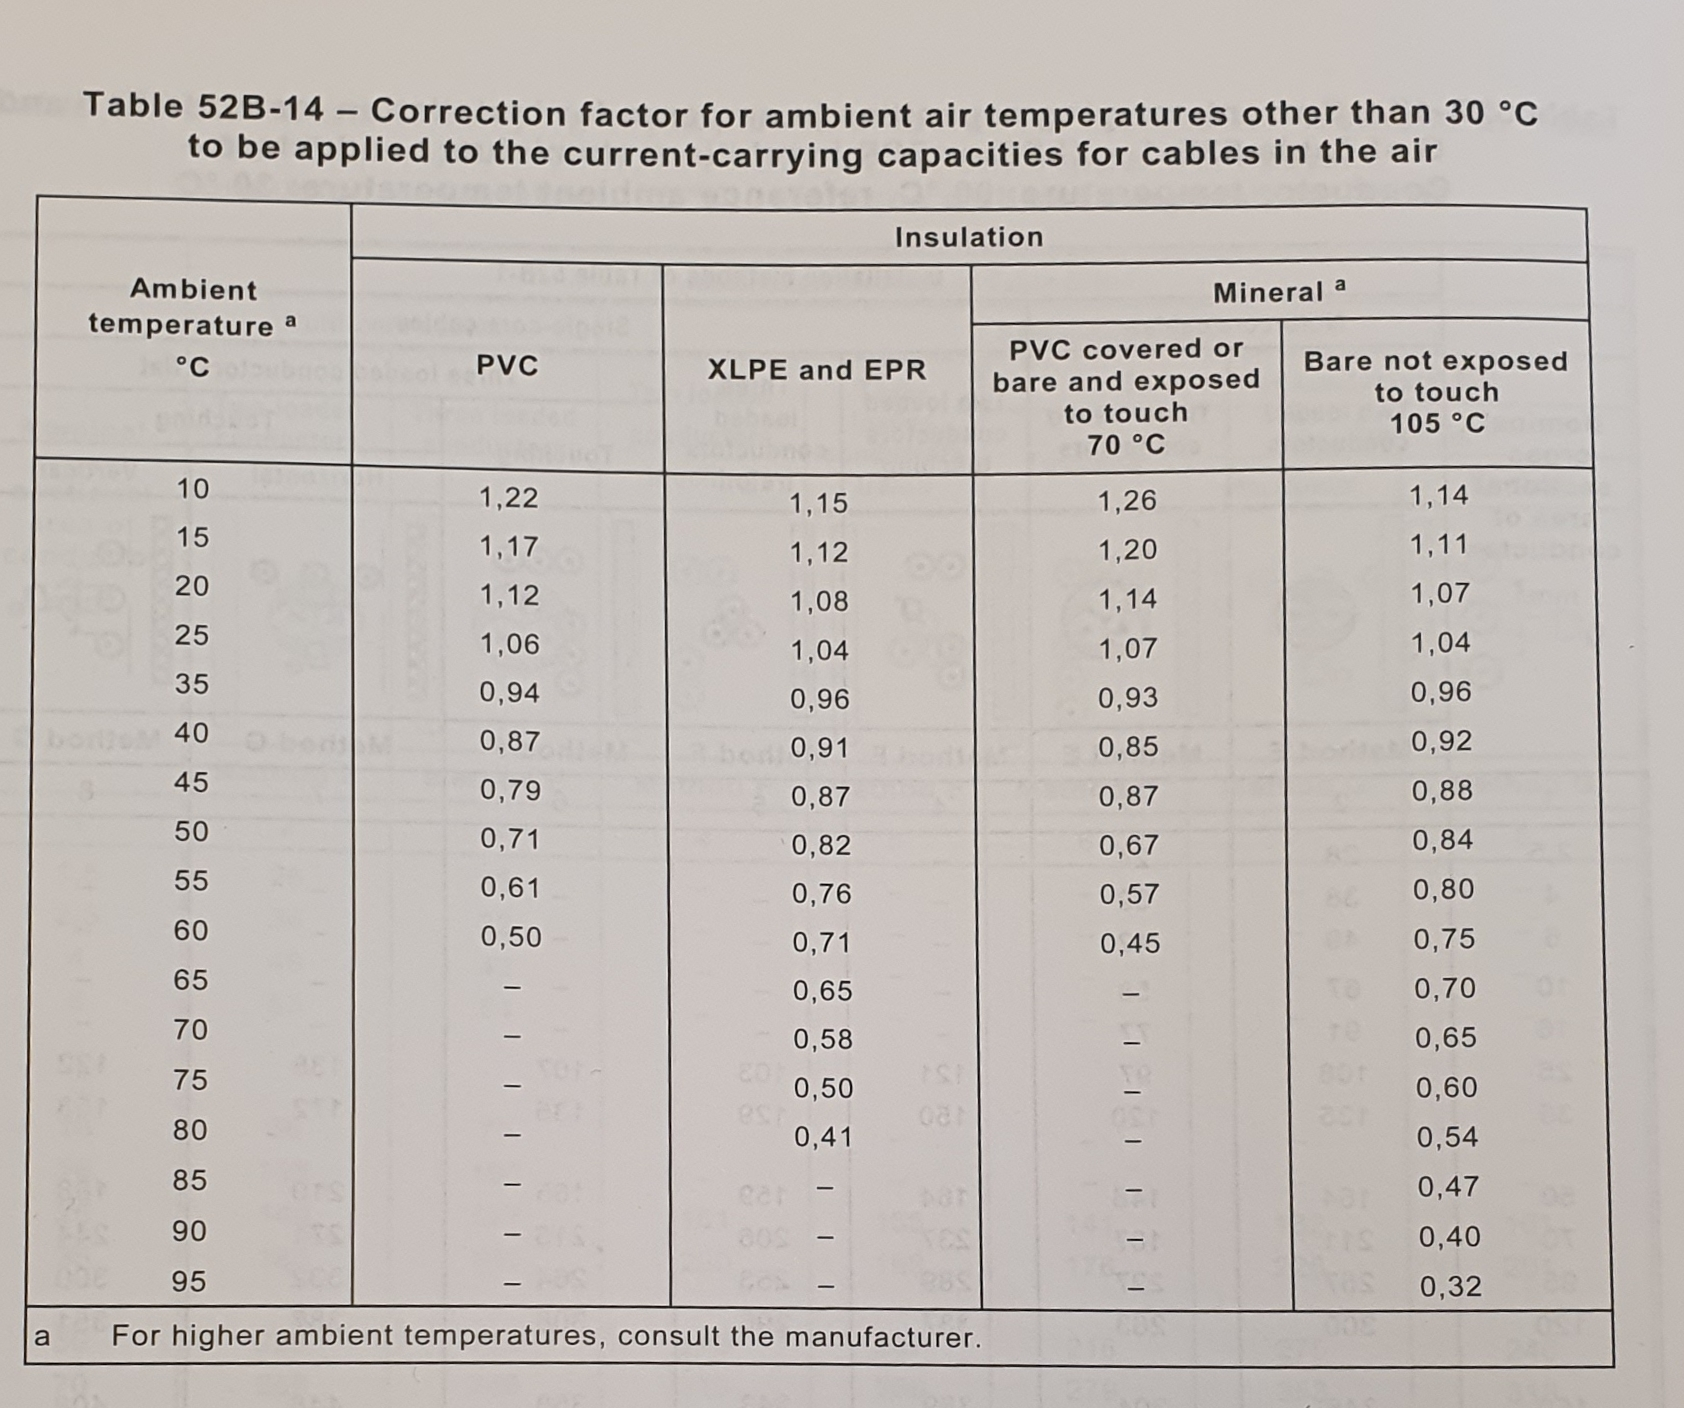
\includegraphics[width=0.9\textwidth]{bilder/temp.jpg}\\

Helt til sist beregnes spenningsfall ved

$\triangle U=\frac{I\cdot \rho \cdot l}{S}$\\
Hvorav\\
$\triangle U$= Spenningsfall i Volt\\
I=strømtrekk\\
$\rho$=Resistivitet [$\Omega \cdot mm^2$]\\
l=total sløyfelengde\\
S=tverrsnitt [$mm^2$]\\
\\
\subsection*{Atmega328p Pinout}
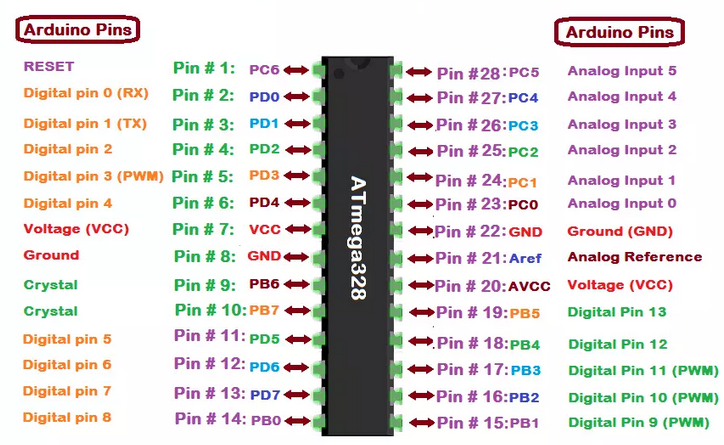
\includegraphics[width=0.9\textwidth]{bilder/Atmega pinout.png}
\newpage
\section*{Oppgave 0: forberedelse}
\subsection*{Håndvask}
Det første og siste steget i alt av laboratoriearbeid er å vaske hender. Hvorfor lurer du kanskje på? På hendene er det et naturlig fettlag, samt annen smuss som kan ha negativ effekt for signalintegritet. Videre motvirker det elektrostatiske utladninger, alle avløp i Norge skal være jordet, ved å vaske hender så reduserer du potensialet mot jord, som i sin tur minsker sannsynligheten for å skade sensitivt utstyr. Ved mer sensitivt utstyr som dere kan møte i studiet vil dere møte krav til EMC-armbånd og hanskebruk.
\subsubsection*{Hent utstyr}


\newpage
\section*{Oppgave 1: Skjemateknikk}
Tegn følgende krets:
12vDC kilde skal forsyne en effektmotstand på $2\Omega$. Kretsen skal inneholde en startbryter med låsende dreiebetjening og nødstoppbryter. Spenningskilde, betjening og nødstopp er i eget skap. Effektmotstanden skal kunne tas ut av kretsen, og det er 5m mellom skap og motstand.
Det tillates en nedre spenning på 11vDC ved effektmotstanden. Kabeldimmensjon skal beregnes.

Anta ingen tap i tilkoblingspunkter, og at ledningssløyfen i skapet er neglisjerbar.

\section*{Oppgave 2: Kabelberegninger Arduino}
Arduino Uno har et maksimalt strømtrekk på 200mA. Beregn minste kabelstørrelse [$mm^2$] som innfrir tekniske krav, se bort fra spenningsfall.

Ut fra beregningene, ta stilling til når man burde kontrollregne på dimmensjoner.

\section*{Oppgave 3: Kabelberegninger breadboard}
En vanlig praksis ved breadboards og prototypearbeid er å bruke dupont ledninger (jumper wires) de er typisk 22awg, eller 0.33$mm^2$.

Beregn spenningsfallet ved 10, 25 og 50cm

\section*{Oppgave 4: Arduino as ISP og bootloader}
Dere skal nå lage en \emph{mvp} (Minimum Viable Product) versjon av en Arduino Uno.
For å oppnå dette så benytter man en Arduino som \emph{ISP} (In-System Programming) Dette tillater å programmere mikrokontrollerne tilkoblet den ferdige kretsen.

Det første steget er å skrive bootloader. Bootloaderens funksjon er å motta instruksjoner, og flytte de til minneposisjoner der de tilgjengeliggjøres for mikrokontrolleren. Før dette stadiet innehar altså ikke mikrokontrolleren nødvendig informasjon for å motta instruksjoner. 

\subsection*{Oppkobling Atmega}
\begin{center}
    \begin{longtable}{||c|c||}
    \cline{1-2}
    Komponent & Atmega Pin\\
    \cline{1-2}
    \cline{1-2}
    5V & 7\\
    \cline{1-2}
    5V & 20\\
    \cline{1-2}
    Gnd & 8\\
    \cline{1-2}
    Gnd & 22\\  
    \cline{1-2}
    220 $\Omega$ ben A & 1\\
    \cline{1-2}
    220 $\Omega$ ben B & 8\\
    \cline{1-2}
    16MHz krystall ben 1 & 9\\
    \cline{1-2}
    16MHz krystall ben 2 & 10\\
    \cline{1-2}
    22pF nr. 1 ben 1 & 8\\
    \cline{1-2}
    22pF nr. 1 ben 2 & 9\\
    \cline{1-2}
    22pF nr. 2 ben 1 & 8\\
    \cline{1-2}
    22pF nr. 2 ben 2 & 10\\
    \cline{1-2}
    \end{longtable}
\end{center}
\subsection*{Oppkobling Arduino - Atmega}
\begin{center}
    \begin{longtable}{||c|c||}
    \cline{1-2}
    Arduino Pin & Atmega 328p Pin\\
    \cline{1-2}
    \cline{1-2}
    10 & 1\\
    \cline{1-2}
    11 & 17\\
    \cline{1-2}
    12 & 18\\
    \cline{1-2}
    13 & 19\\
    \cline{1-2}
    \end{longtable}
\end{center}

Koble Arduino til PC, åpne Arduino IDE.
\begin{enumerate}
    \item  Tools $\rightarrow$ Board $\rightarrow$ Arduino Uno
    
    \item File $\rightarrow$ Examples $\rightarrow$ ArduinoISP $\rightarrow$ ArduinoISP $\rightarrow$ Upload
    
    \item Tools $\rightarrow$ Programmer $\rightarrow$ Arduino as ISP $\rightarrow$ burn bootloader
\end{enumerate}

Etter å ha skrivet til bootloaderen kan man koble fra alle oppkoblingene i Oppkobling Arduino - Atmega

\section*{Oppgave 5: Arduino som ttl}
Koble Arduinoens reset pin til Gnd. Med dette tvinges mikrokontrolleren på Arduino av, og vi kan dermed benytte den for å konvertere USB til Seriell.

\subsection*{Oppkobling Arduino - Atmega}
\begin{center}
    \begin{longtable}{||c|c||}
    \cline{1-2}
    Arduino Pin & Atmega 328p Pin\\
    \cline{1-2}
    \cline{1-2}
    RX & 2 \\
    \cline{1-2}
    TX & 3 \\
    \cline{1-2}
    \end{longtable}
\end{center}

\section*{Oppgave 6: Blink led}
Nå kan man programmere Atmega328p som en vanlig arduino. Dere skal lage et enkelt program som blinker en lysdiode, koble til lysdioden og last opp programmet. NB! ved opplastning så må Atmegaen resettes ved start av opplastning. Dette oppnår man med å kortslutte Gnd og pin 1 ved start av opplastning.
\end{document}

